\section{Фазовый синхронизм при фотоиндуцированной генерации второй 	гармоники в оптическом волокне}

\begin{frame}
	\frametitle{Кривые фазового синхронизма при ГВГ в оптических волокнах}
	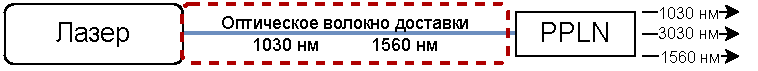
\includegraphics[width=\linewidth]{Presentation/images/problem_fiber}
	
	\fixme{Сжатая мотивация исследования, модели, приход к кривім}
	
	\begin{columns}
		\begin{column}{0.49\textwidth}			
			\fixme{ЛК, ПРЛК}
			
		\end{column}
		\begin{column}{0.45\textwidth}
			\fixme{какая-то картинка}
		\end{column}
	\end{columns}	
\end{frame}

\begin{frame}
	\frametitle{Кривые фазового синхронизма при ГВГ в оптических волокнах}
	\framesubtitle{Эксперимент}

	
	\begin{columns}
		\begin{column}{0.46\textwidth}			
			Методика эксперимента:
			
			\begin{itemize}
				\item Запись решётки второй  гармоники; $P_{\text{pump}}=38~\text{Вт}$;
				
				\item По достижении определённой мощности второй гармоники процесс записи приостанавливается и производится измерение кривых спектрального и температурного (температура волокна) синхронизмов; $P_{\text{pump}}=500~\text{мВт}$;
				
				\item Процесс записи на мощности накачки $P_{\text{pump}}=38~\text{Вт}$ продолжается. 
			\end{itemize}
			
		\end{column}
		\begin{column}{0.54\textwidth}
			\centering
			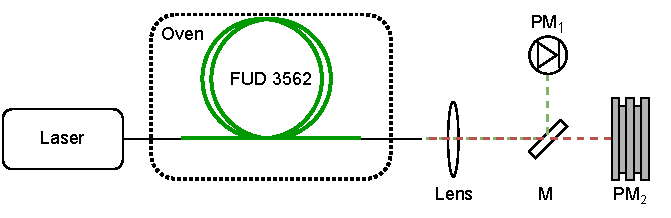
\includegraphics[width=0.9\linewidth]{Dissertation/images/fibershg/scheme}
				
			\footnotesize{Экспериментальная установка. M: дихроичные зеркала; PM$_1$, PM$_2$: измерители мощности}
			
			\vfill
			
			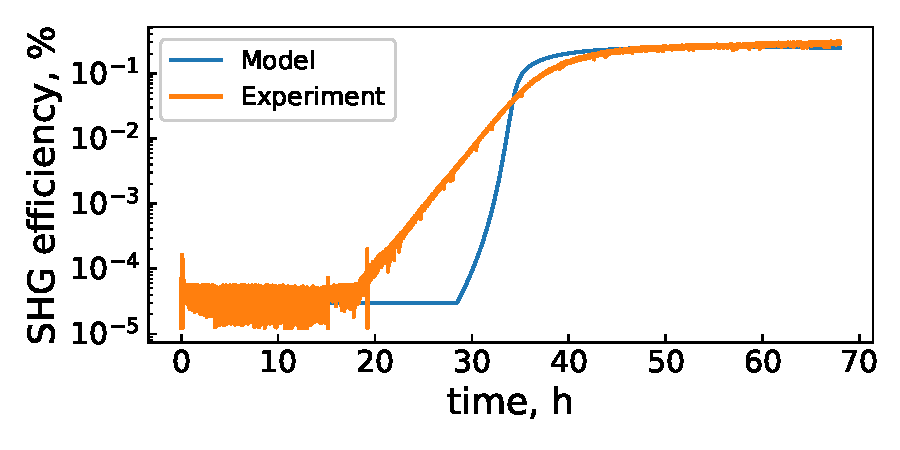
\includegraphics[width=0.9\linewidth]{Dissertation/images/fibershg/kinetic}
			
			\footnotesize{Эффективности ГВГ от времени. Оранжевый: эксперимент, синий: моделирование.}
		\end{column}
	\end{columns}	
\end{frame}

\begin{frame}
	\frametitle{Кривые фазового синхронизма при ГВГ в оптических волокнах}
	\framesubtitle{Модель}
	\fixme{Уравнения взял из Антонюка\footnote{Антонюк Б. П., Антонюк В. Б. Самоорганизация возбуждений в германосиликатных волоконных световодах и ее роль в генерации второй гармоники //Успехи физических наук. – 2001. – Т. 171. – №. 1. – С. 61-78.}}
	
	\begin{columns}
		\begin{column}{0.6\textwidth}			
			\fixme{уравнения}
			
		\end{column}
		\begin{column}{0.4\textwidth}
			\fixme{расшифровки}
		\end{column}
	\end{columns}	
\end{frame}

\begin{frame}
	\frametitle{Кривые фазового синхронизма при ГВГ в оптических волокнах}
	\framesubtitle{Результаты}
	
	\centering
	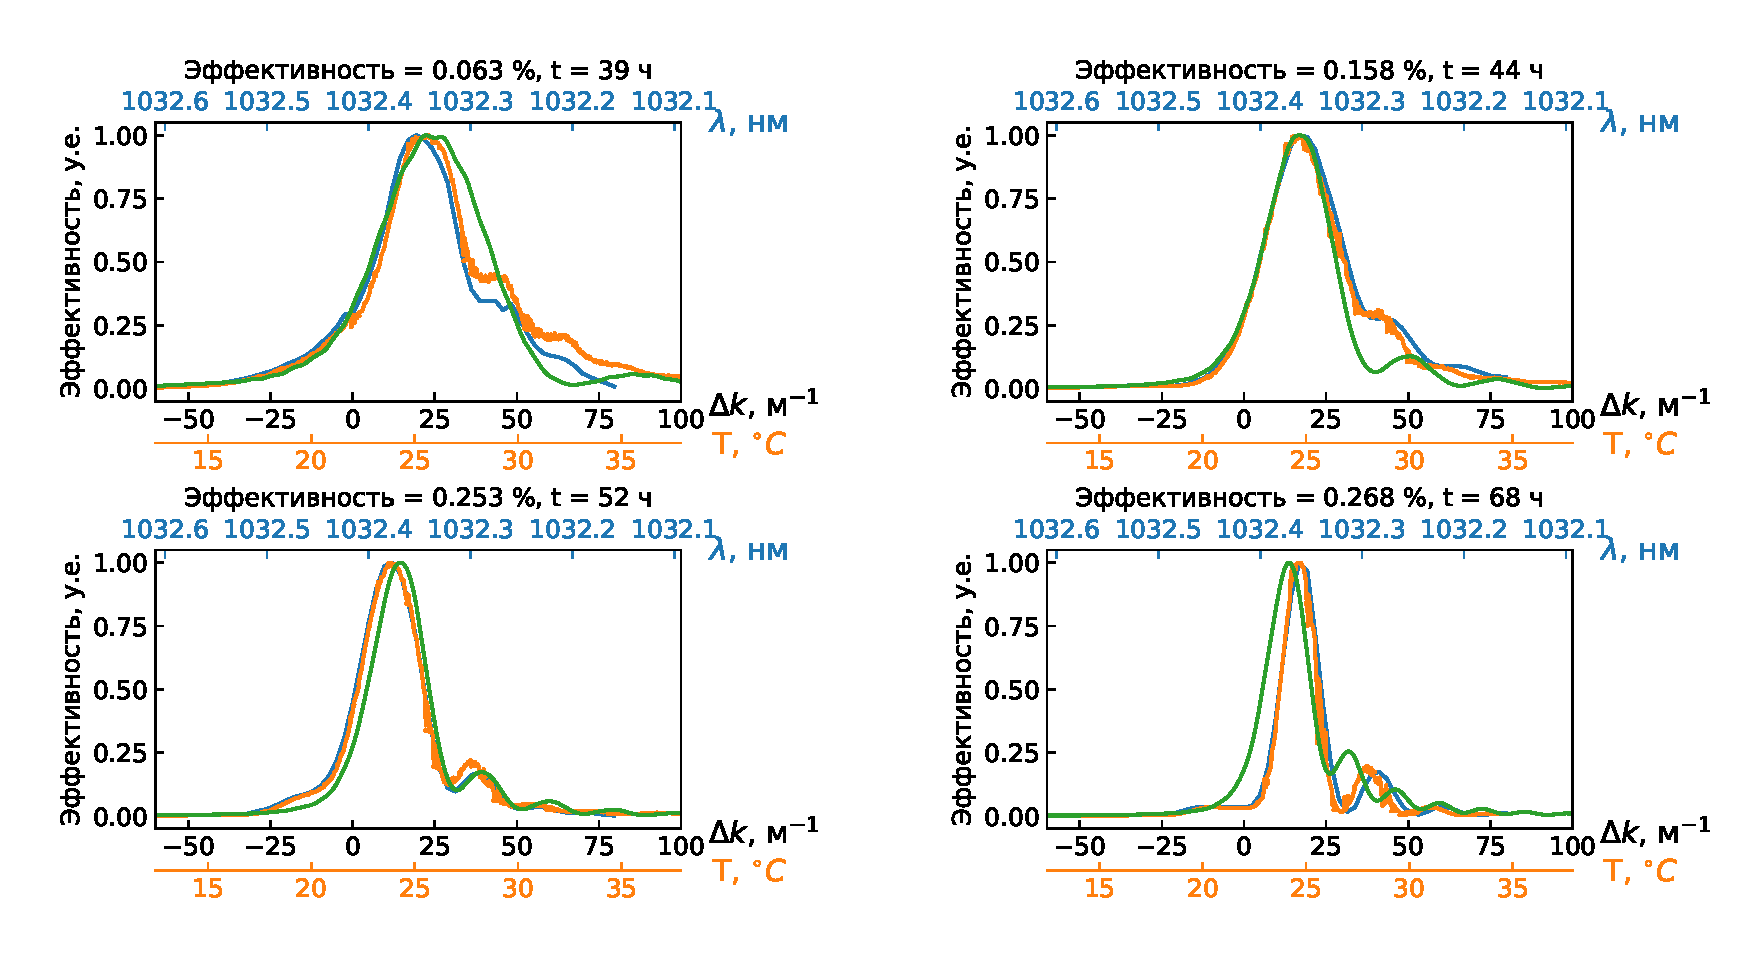
\includegraphics[width=0.8\linewidth]{Dissertation/images/fibershg/curves}
	
	\footnotesize{КФС, измеренные на различных этапах записи \(\chi^{(2)}\)-решётки. Синие и оранжевые кривые соответствуют спектральному и температурному фазовым синхронизмам соответственно, зелёные~--- результат моделирования}
	
\end{frame}

\begin{frame}
	\frametitle{Кривые фазового синхронизма при ГВГ в оптических волокнах}
	\framesubtitle{Результаты}
	
	\centering
	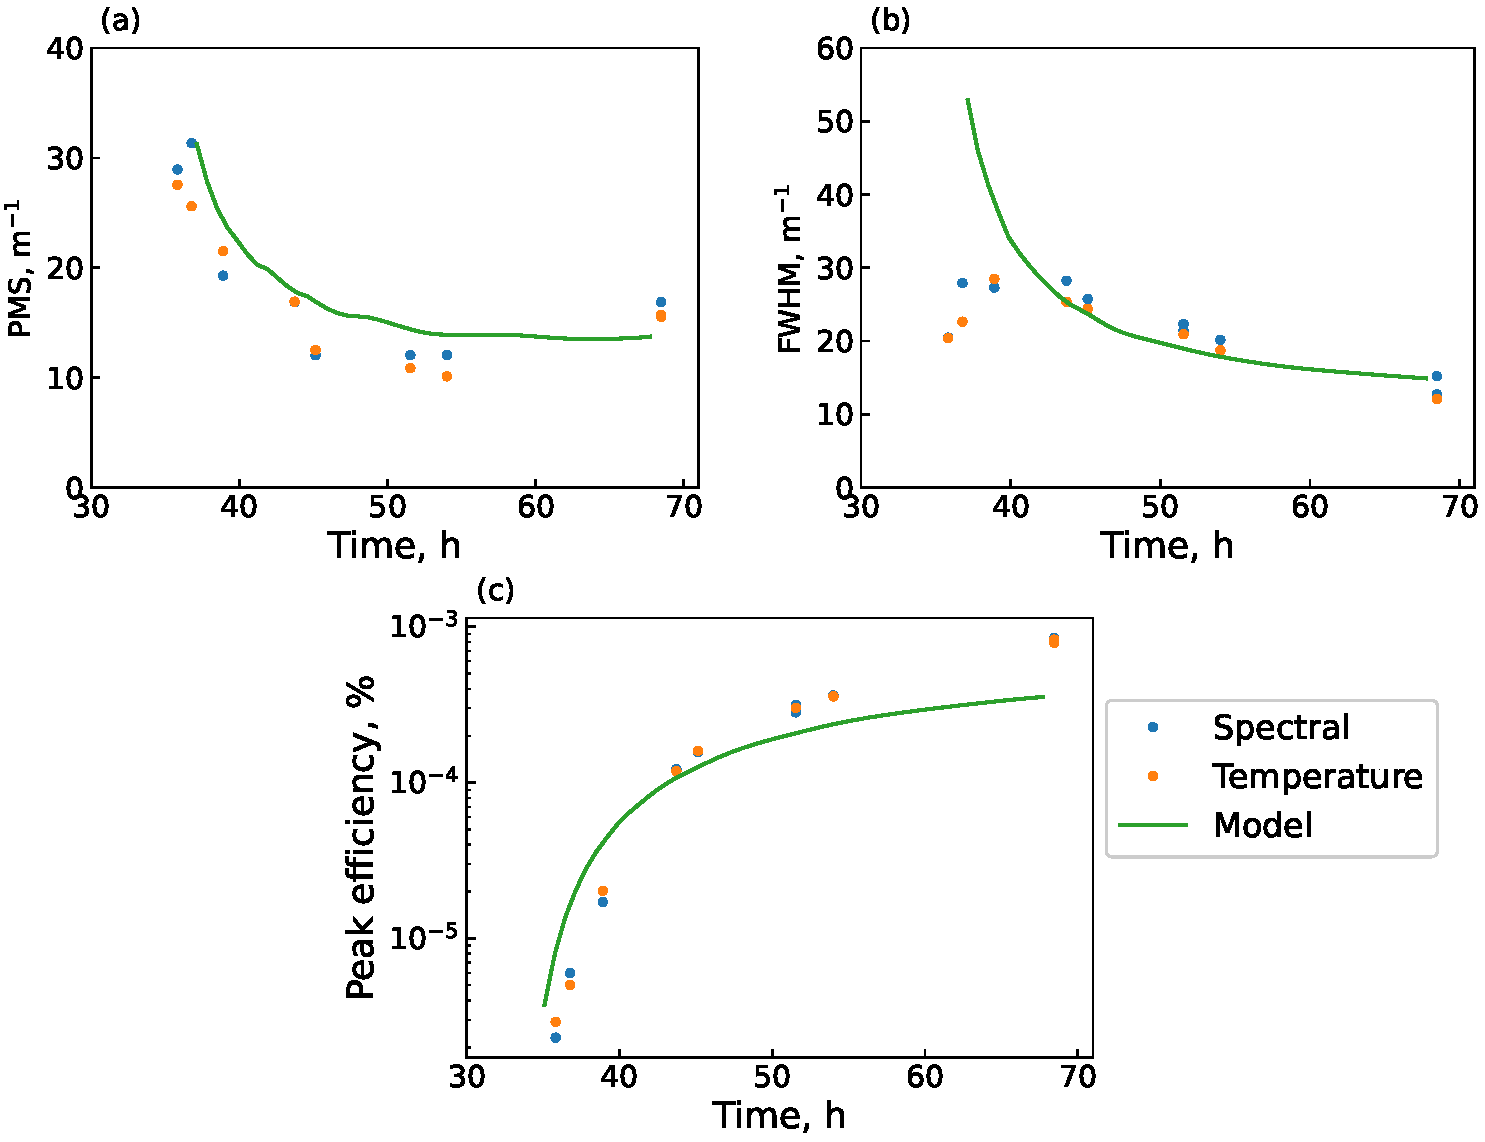
\includegraphics[width=0.6\linewidth]{Dissertation/images/fibershg/mc_dk}
	
	\footnotesize{Кинетики сдвига фазового синхронизма (СФС) (a), ширины кривой на половине высоты (FWHM) (б) и пиковой эффективности в процессе формирования \(\chi^{(2)}\)-решётки (в). Синие и оранжевые точки — экспериментальные значения, полученные при измерениях спектральных и температурных КФС соответственно, зеленые кривые — результаты моделирования}
	
\end{frame}



